\documentclass{article}
\usepackage{amsmath}
\usepackage{amssymb}
\usepackage{indentfirst}
\usepackage{graphicx}
\usepackage{color}
\usepackage{fancyhdr}
\usepackage{epstopdf}
\usepackage{indentfirst}
\usepackage{geometry}
\geometry{left=2.5cm,right=2.5cm,top=2.5cm,bottom=2.5cm}

\title{14.03 Problem Set 3}
\author{Yijun Jiang}
%\email{yjjiang@mit.edu}
\date{\today}

\pagestyle{fancy}
\lhead{Yijun Jiang}
\rhead{14.03 Problem Set 3}

\begin{document}
\maketitle

\section{Tariffs and Quotas}
\subsection{Part 1}
If US does not trade with the rest of world, domestic demand should balance domestic supply.
\begin{align*}
	&P=2+Q\\
	&Q=-\frac{1}{3}P+6
\end{align*}
whose solution is $P^*=6$ and $Q^*=4$. This is the equilibrium price and quantity in autarky.

\subsection{Part 2}
The new supply curve first goes as $P=2+Q$ and then becomes perfectly elastic at $P=3$. Once $Q$ is large enough to make $P=3$, Chinese suppliers enter the market and fixes market price at $P=3$. For US suppliers, only those who are willing to supply at $P\leqslant3$ can survive in this market. In the previous part we find that $P=6>3$. Therefore, we know that Chinese suppliers do enter the market. The new equilibrium price is then $P^*=3$, both for US and Chinese suppliers. The equilibrium quantity is given by the domestic demand function, $Q^*=-\frac{1}{3}P+6=5$.

At the turning point where Chinese suppliers enter the market, $Q^*_{US}=P^*-2=1$. This is the quantity produced by US suppliers. The rest of the demand, $Q^*_{CHN}=Q^*-Q^*_{US}=4$, is imported from Chinese suppliers.

\subsection{Part 3}
This tariff effectively sets the Chinese supply curve to $P=3+t=4.5$, which is still lower than $P=6$ found in part 1. So Chinese suppliers still enter the market and market price will be fixed at $P^*=4.5$, but more US suppliers can sell their T-shirts at this higher price. Numerically, $Q^*_{US}=P^*-2=2.5$.

In conclusion, the equilibrium price and quantity sold by US manufacturers are now $P^*=4.5$ and $Q^*_{US}=2.5$. So $\Delta P^*=1.5$ and $\Delta Q^*_{US}=1.5$.

\subsection{Part 4}
The US manufacturers who can supply below $P=3$ (low-cost US suppliers) enter the market first, then Chinese suppliers, and finally, when the import quota is used up but consumers still demand more T-shirts, the price is raised above $P=3$ and the rest US suppliers (high-cost US suppliers) enter the market.

In order to maintain the domestic production level, the equilibrium price must be $P^*=2+Q^*_{US}=4.5$. At this price, domestic demand is $Q^*=-\frac{1}{3}P+6=4.5$. So the quota must be set as $Q^*_{CHN}=Q^*-Q^*_{US}=2$.

\subsection{Part 5}
See Fig.\ref{DandS} for the graph.
\begin{figure}[!htbp]
	\centering
	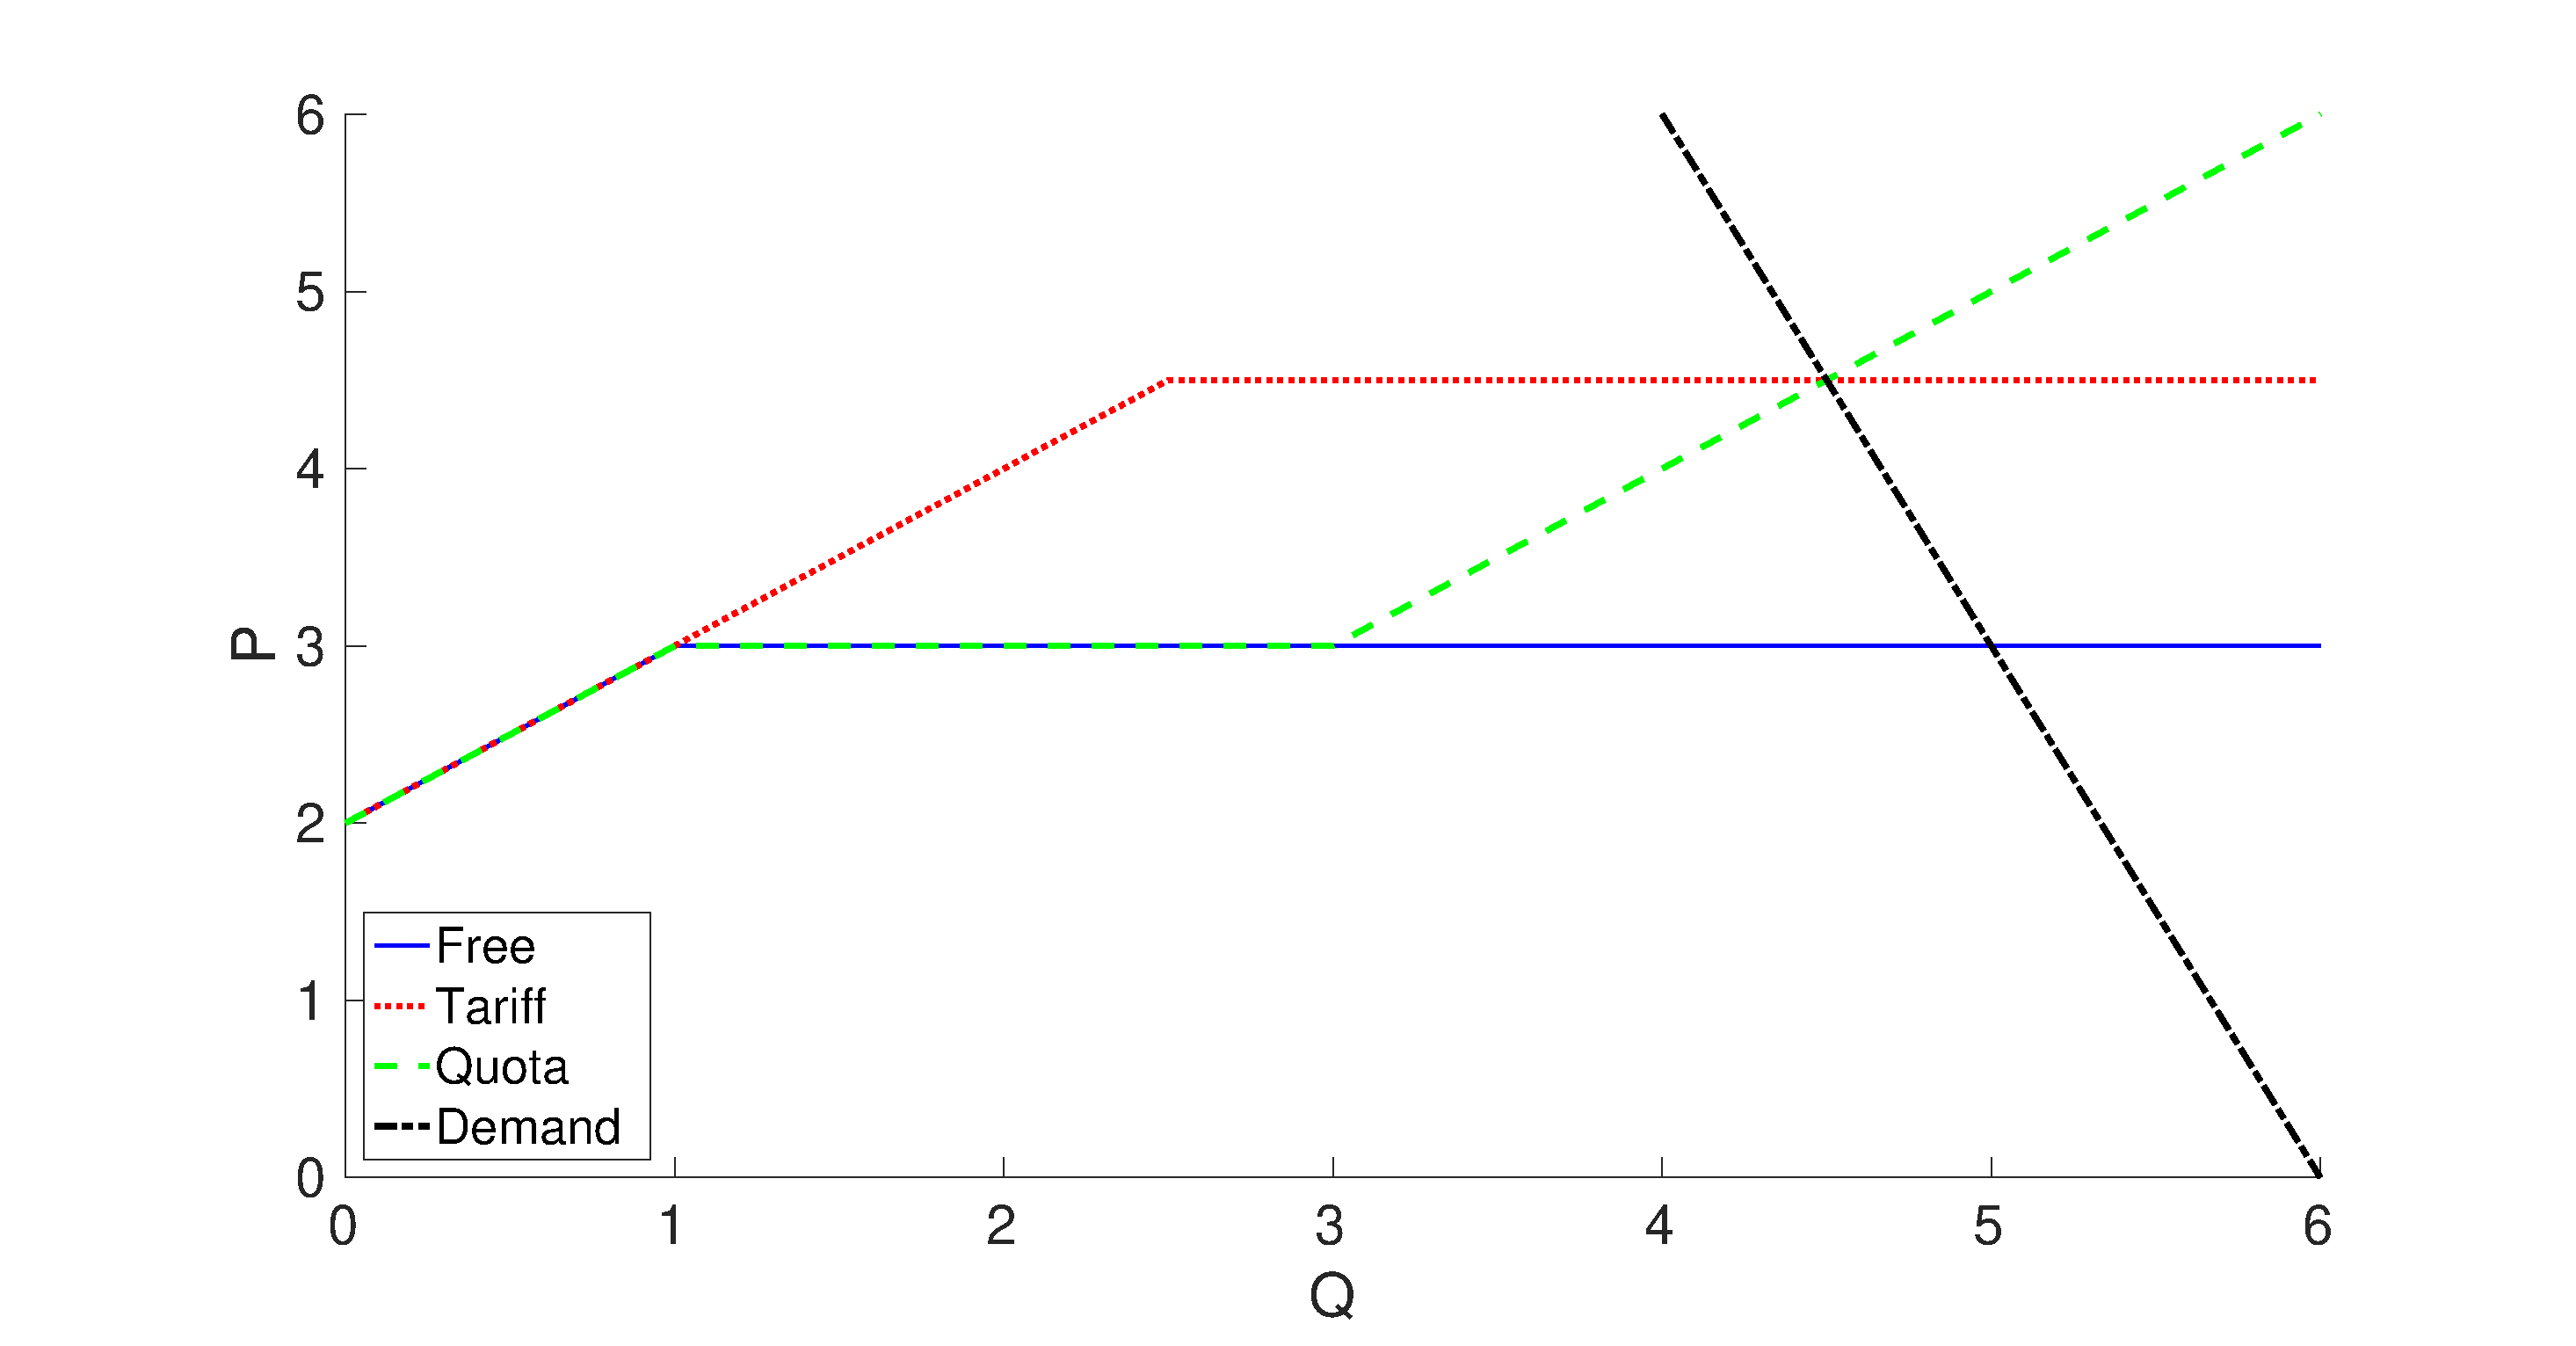
\includegraphics[width=12cm]{figure1.eps}\\
	\caption{Demand and supply curves of free trade and trade with tariff or quota}
	\label{DandS}
\end{figure}

\subsection{Part 6}
See Fig.\ref{surplus} for a graphical illustration.
\begin{figure}[!htbp]
	\centering
	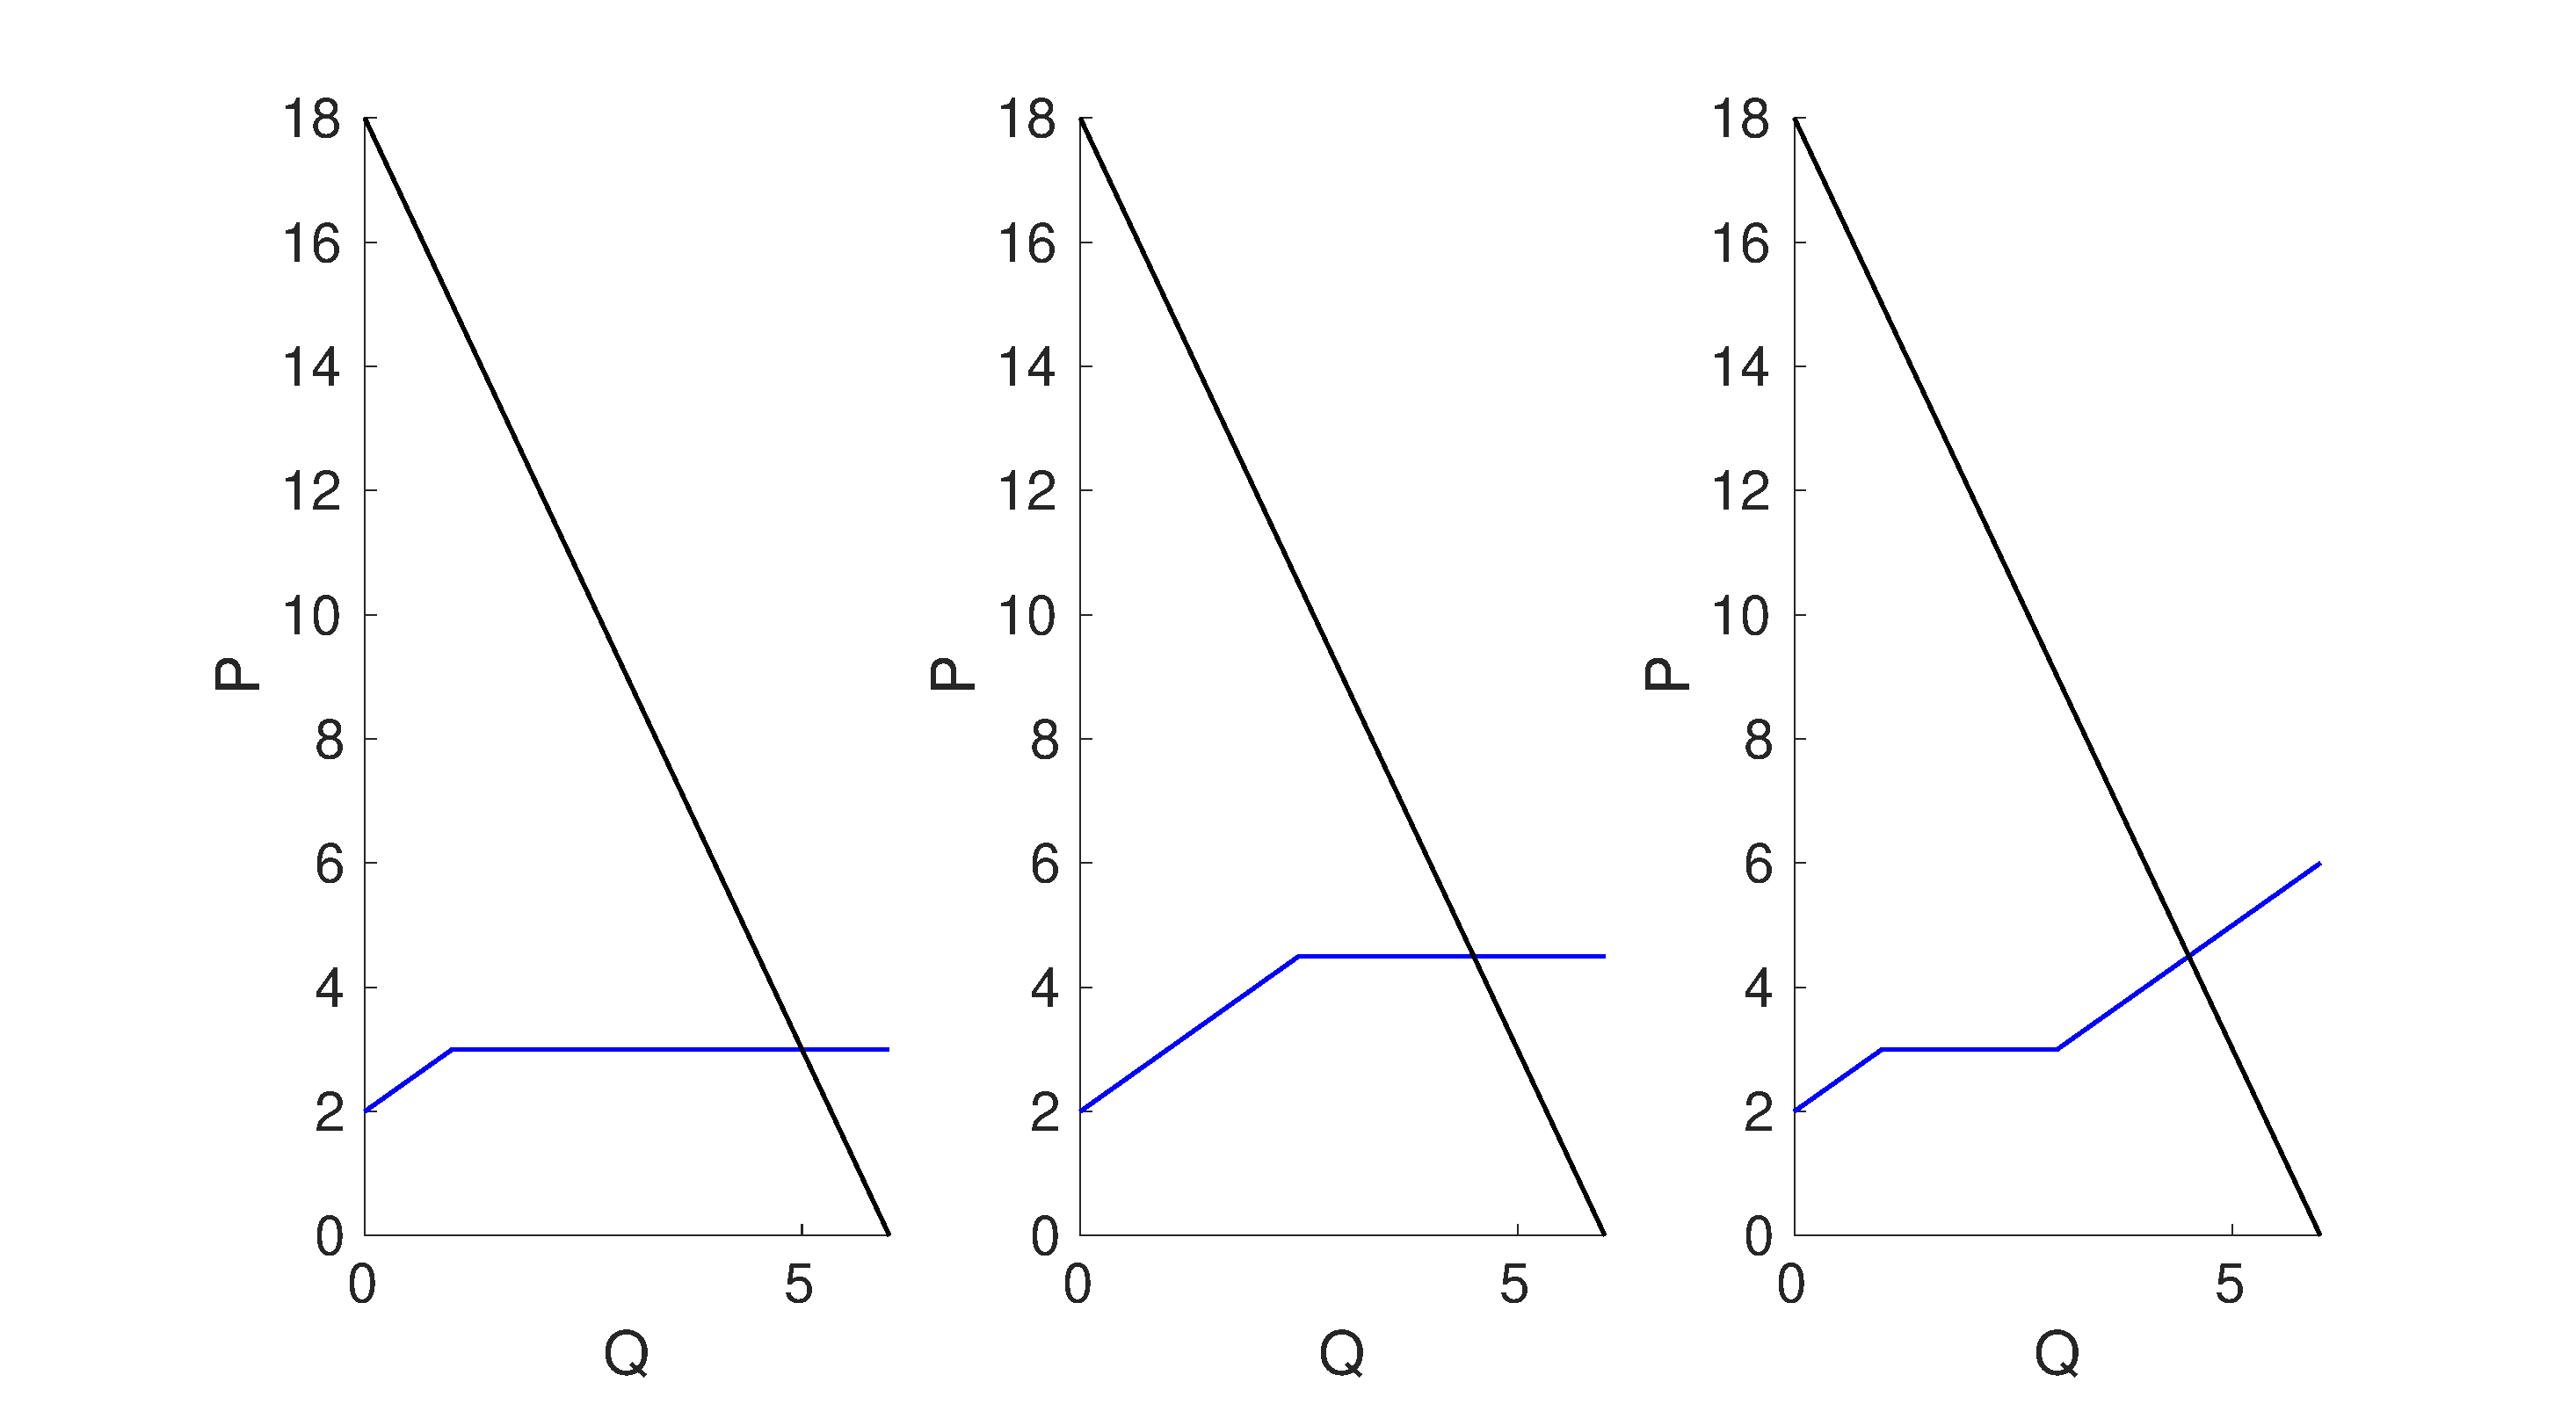
\includegraphics[width=12cm]{figure2.eps}\\
	\caption{Consumer and producer surplus of (left) free trade, (middle) trade with tariff, and (right) trade with quota}
	\label{surplus}
\end{figure}

In the free trade regime, consumer surplus is the area of the large triangle. US producer surplus is the area of the small triangle, while Chinese suppliers do not have any producer surplus. US government does not have any revenue.
\begin{align*}
&CS_{free}=5\times(18-3)/2=37.5\\
&PS_{US,free}=1\times(3-2)/2=0.5\\
&PS_{CHN,free}=0\\
&GR_{free}=0
\end{align*}

In the tariff regime, consumer surplus is the area of the large triangle. US producer surplus is the area of the small triangle, while Chinese suppliers do not have any producer surplus. US government revenue is the area of the rectangle.
\begin{align*}
&CS_{tariff}=4.5\times(18-4.5)/2=30.375\\
&PS_{US,tariff}=2.5\times(4.5-2)/2=3.125\\
&PS_{CHN,tariff}=0\\
&GR_{tariff}=(4.5-2.5)*(4.5-3)=3
\end{align*}


In the quota regime, consumer surplus is the area of the large triangle. US producer surplus has two parts on the graph: one for low-cost suppliers and the other for high-cost suppliers. Chinese producer surplus is the area of the rectangle. US government does not have any revenue.
\begin{align*}
&CS_{quota}=4.5\times(18-4.5)/2=30.375\\
&PS_{US,quota}=1\times((4.5-2)+(4.5-3))/2+(4.5-3)\times(4.5-3)/2=3.125\\
&PS_{CHN,quota}=(3-1)\times(4.5-3)=3\\
&GR_{quota}=0
\end{align*}

US consumers get the largest surplus in the free trade, so they prefer no import constraints. US producers regard both tariff and quota as better than free trade, and they are indifferent between tariff and quota policy, as long as the two policies give them the same market share. Chinese producers will prefer quota to tariff, for they get some producer surplus in the quota regime, which in the tariff regime turns into US government revenue.

\section{Deadweight Loss of Taxation}
\subsection{Part 1}
The utility maximization problem is
\begin{align*}
&u^*=\max_{x,y}\{u(x,y)=x^{2/3}y^{1/3}\}\\
&\textup{s.t. }xP_x+yP_y=I
\end{align*}

The Lagrangian is $L(x,y,\lambda)=x^{2/3}y^{1/3}+\lambda(I-xP_x-yP_y)$. Setting partial derivatives to zero,
\begin{align*}
&\frac{2}{3}\left(\frac{x}{y}\right)^{-1/3}=\lambda P_x\\
&\frac{1}{3}\left(\frac{x}{y}\right)^{2/3}=\lambda P_y\\
&xP_x+yP_y=I
\end{align*}
whose solution is
\begin{align*}
x&=\frac{2I}{3P_x}\\
y&=\frac{I}{3P_y}\\
\lambda&=\frac{1}{3}\left(\frac{1}{4}P_x^2P_y\right)^{-1/3}
\end{align*}

This gives the uncompensated demands,
\begin{align*}
d_x(P_x,P_y,I)&=\frac{2I}{3P_x}\\
d_y(P_x,P_y,I)&=\frac{I}{3P_y}
\end{align*}
as well as the indirect utility function,
\begin{equation*}
V(P_x,P_y,I)=u(d_x,d_y)=\frac{2^{2/3}}{3}P_x^{-2/3}P_y^{-1/3}I
\end{equation*}

\subsection{Part 2}
Since utility remains the same, we have
\begin{equation*}
V(P_x,P_y,I)=V(P_x(1+t),P_y,I+\delta I)
\end{equation*}

In other words,
\begin{align*}
\frac{2^{2/3}}{3}P_x^{-2/3}P_y^{-1/3}I&=\frac{2^{2/3}}{3}(P_x(1+t))^{-2/3}P_y^{-1/3}(I+\delta I)\\
\delta I&=\left((1+t)^{2/3}-1\right)I
\end{align*}

\subsection{Part 3}
\begin{align*}
TR&=tP_x\cdot d_x(P_x(1+t),P_y,I+\delta I)\\
&=tP_x\frac{2(I+\delta I)}{3P_x(1+t)}\\
&=\frac{2I}{3}\frac{t}{(1+t)^{1/3}}
\end{align*}

\subsection{Part 4}
\begin{align*}
DWL&=\delta I-TR\\
&=\left((1+t)^{2/3}-1\right)I-\frac{2I}{3}\frac{t}{(1+t)^{1/3}}\\
&=\frac{(1+t/3)-(1+t)^{1/3}}{(1+t)^{1/3}}I\\
&=\frac{t^2/9-5t^3/81+O(t^4)}{(1+t)^{1/3}}I
\end{align*}

This deadweight loss is zero when $(1+t/3)=(1+t)^{1/3}$, which happens if and only if $t=0$. This is the trivial solution where no taxation exists. Nonzero tax always leads to a positive deadweight loss, for $(1+t/3)>(1+t)^{1/3}$ always holds when $t>0$. In other words, the government needs to rebate more than its tax revenue in order to make consumers equally satisfied as before.

\subsection{Part 5}
The diagram is shown in Fig.\ref{blank}, in which we can see that the cost of the new bundle at the original prices is higher than the original bundle. This intuitively makes sense because according to the dual problem, the original bundle minimizes the expenditure on this indifference curve. This statement is always true as long as $t>0$, so there is always some positive deadweight loss.
\begin{figure}[!htbp]
	\centering
	
\includegraphics[width=12cm]{blank.png}\\
	\caption{Graphical illustration of taxation and rebate}
	\label{blank}
\end{figure}

\section{General Equilibrium in a Pure Exchange Economy}
\subsection{Part 1}
The Edgeworth box is shown in Fig.\ref{Edgeworth}. Feasible allocations are all the points in the rectangular region $0\leqslant x\leqslant8$, $0\leqslant y\leqslant8$. If $x$ and $y$ must take integer values due to indivisibility of the goods, then feasible allocations are all the integer-coordinated grid points in this rectangle. The initial allocation is marked as a circle.
\begin{figure}[!htbp]
	\centering
	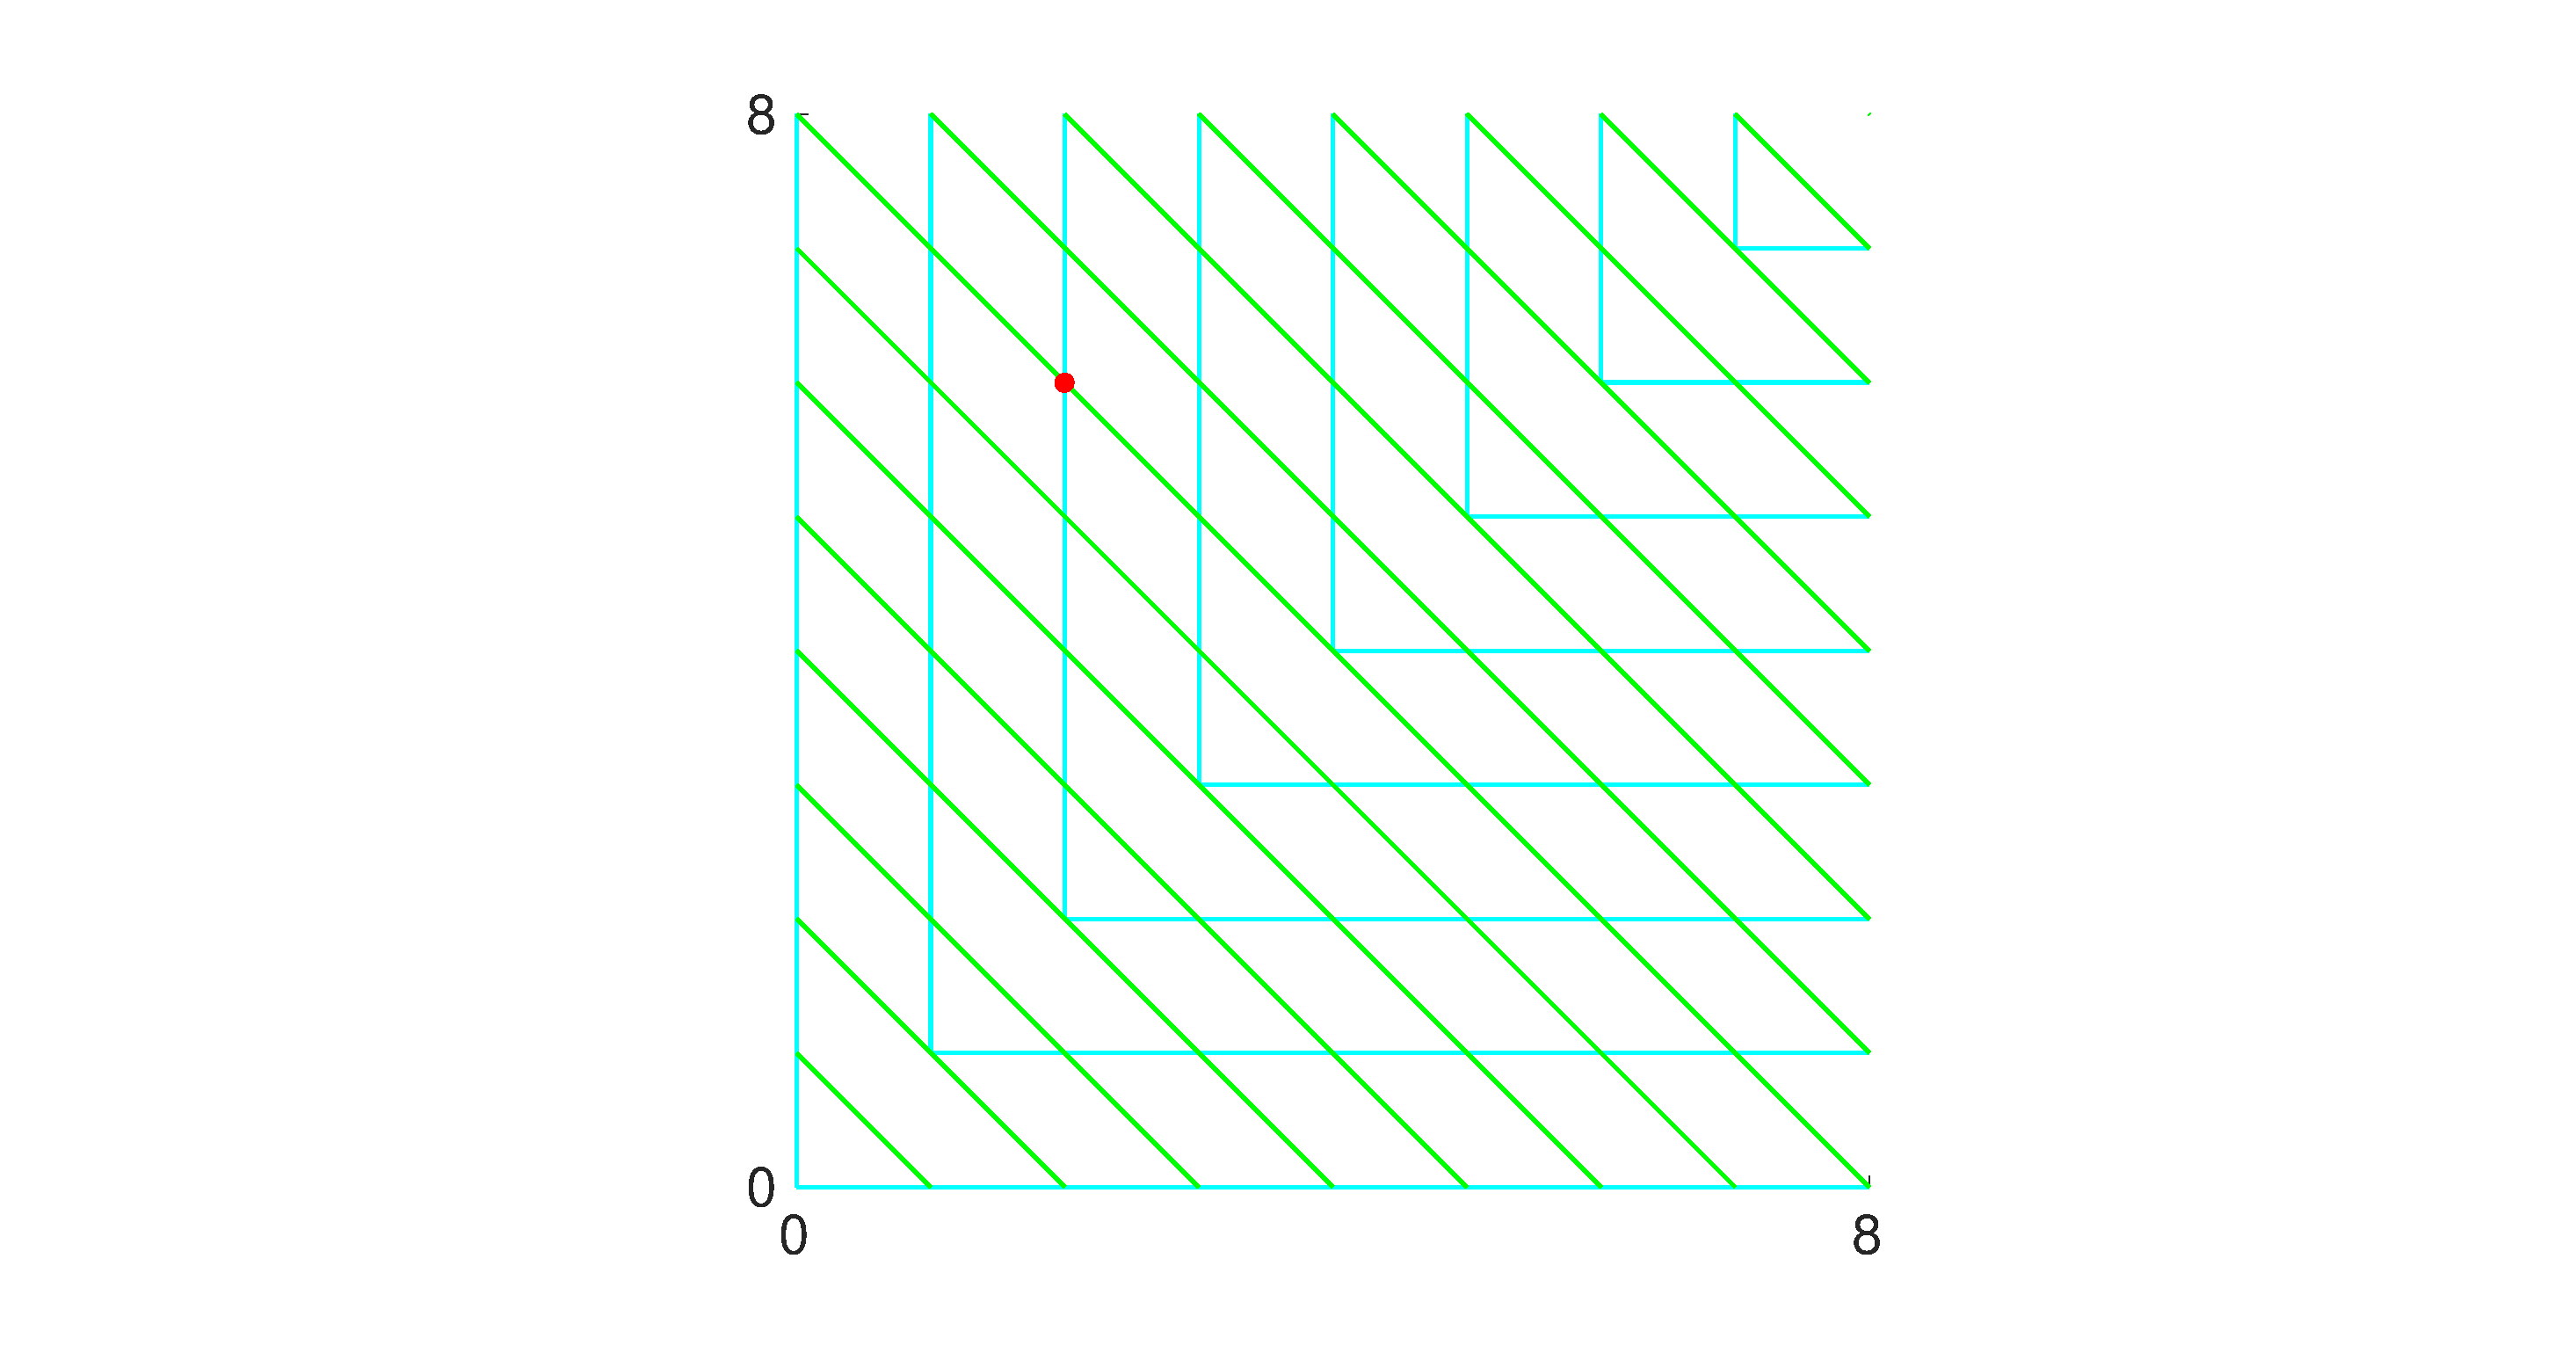
\includegraphics[width=12cm]{figure3.eps}\\
	\caption{Edgeworth box of Ann and Bob}
	\label{Edgeworth}
\end{figure}





\end{document}
